% 前言
\documentclass{article}
\usepackage[UTF8]{ctex}
\usepackage[utf8]{inputenc}
\usepackage[a4paper, margin = 2cm]{geometry}
\usepackage[english]{babel}
\usepackage{fancyhdr}
\usepackage{amssymb}
\usepackage{amsmath}
\usepackage{amsfonts}
\usepackage{natbib}
\usepackage{graphicx}

\pagestyle{fancy}
\fancyhf{}
\lhead{}
\rhead{}
\lfoot{}
\rfoot{}
\cfoot{\thepage}
\renewcommand{\headrulewidth}{1pt}
\renewcommand{\footrulewidth}{1pt}

\newtheorem{problem}{Problem}


\begin{document}

\title{2019第四季度习题集}
\author{王海阳}
\date{\today}
\maketitle
\tableofcontents

    \section{Hatcher problems}
        \begin{problem} 
            (pg 39 problem 16.(c): Unsolved). %TODO: unsolved
            \(X = S^1\times D^2.\), \(A\) is the circle in the following graph,
            Prove that there is no retract form X to A. 
            \begin{center}
                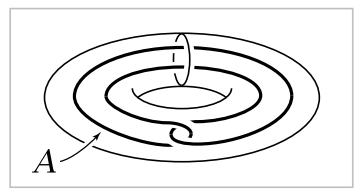
\includegraphics{hatcher习题截图.png}
            \end{center}
        \end{problem}

        \begin{problem}
            (pg 39 problem 16.(d): Unsolved). %TODO: unsolved
            \(X = D^2 \vee D^2\), \(A = S^1 \vee S^1\). 证明没有X到A的retract
        \end{problem}

        \begin{problem}
            
        \end{problem}





\bibliographystyle{plain}
\bibliography{references}
\bibliography{}
\end{document}